\documentclass[a4paper, 10pt, final, garamond]{book}
\usepackage{cours-preambule}

\titleformat{\item}{}{\arabic{item})}{.5em}{}{}
\titleformat{\subitem}{}{\arabic{item}) \alph{subitem} --}{.5em}
{}{}

\makeatletter
\renewcommand{\@chapapp}{Devoir surveill\'e -- num\'ero}
\makeatother

\begin{document}
\setcounter{chapter}{5}

\chapter{Commentaires sur le DS n\degree6}

\begin{NCprop}[width=\linewidth]{\centering\bfseries\ Rappel des malus}
    Chacune des lettres suivantes sur vos copies sont des malus de \num{1}
    point.\smallbreak
    \begin{minipage}{0.50\linewidth}
        \begin{itemize}
            \item A~: application numérique mal faite~;
            \item V~: confusion ou oubli de vecteurs~;
            \item P~: prénom sur copies manquant~;
            \item C~: grands carreaux~!~;
        \end{itemize}
    \end{minipage}
    \begin{minipage}{0.50\linewidth}
        \begin{itemize}
            \item U~: unité manquante ou mauvaise~;
            \item H~: homogénéité non respectée~;
            \item S~: chiffres significatifs non respectés~;
            \item $\f$~: loi physique fondamentale brisée.
        \end{itemize}
    \end{minipage}
\end{NCprop}

\section{Commentaires généraux}

DS à 46, le plus raté de l'année. L'écart se creuse. Moyenne à 09/20. Ne perdez
pas le cap~! Total malus~: \textbf{75}, \underline{bravo} c'est enfin moins que
les points de la meilleure copie. On compte aussi 10 personnes sans un seul
malus, pour un total de \textbf{15.5} points de bonus.

\begin{itemize}
    \item Configuration de \textbf{valence} n'est \textbf{pas} la configuration
        électronique totale~!!
    \item Concentrez-vous sur le lien entre position dans le tableau et
        configuration électronique.
    \item J'ai failli introduire un malus O pour octet… \textbf{vérifiez-vous}.
    \item Il est impensable de passer outre la mécanique~!
    \item Il est \textbf{indispensable} de savoir calculer des produits
        vectoriels.
\end{itemize}

\begin{center}
    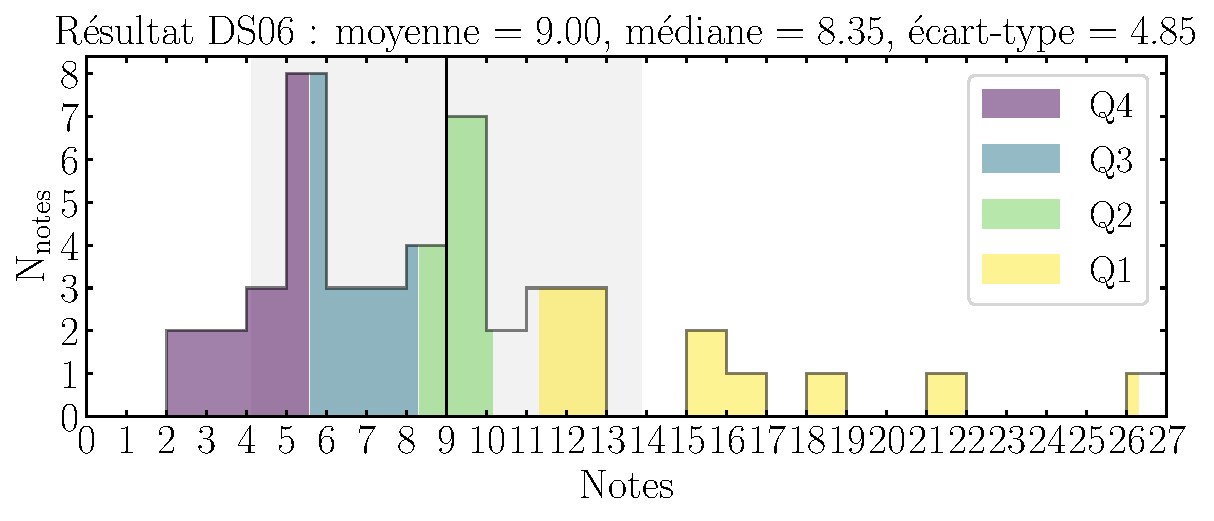
\includegraphics[width=.8\linewidth]{res_DS06.pdf}
\end{center}
\vspace*{-20pt}

\section{Exercice 1 \hfill \textcolor{red}{/32}}
\begin{enumerate}
    \item Composition = protons, neutrons, électrons. Donner la position.
        Configuration de valence $\neq$ configuration totale. Schémas de
        \textsc{Lewis}~: électrons célibataires, pas liaisons covalentes, et
        doublets non-liants, pas deux électrons célibataires l'un à côté de
        l'autre.
        \hfill \textcolor{ForestGreen}{/8}
    \item Cf.\ corrigé.
        \hfill \textcolor{ForestGreen}{/2}
    \item Cf.\ corrigé.
        \hfill \textcolor{ForestGreen}{/3}
    \item Cf.\ corrigé.
        \hfill \textcolor{ForestGreen}{/5}
    \item Cf.\ corrigé.
        \hfill \textcolor{ForestGreen}{/4}
    \item Cf.\ corrigé.
        \hfill \textcolor{ForestGreen}{/2}
    \item Il faut savoir traduire «~cyclique~». Ça n'est pas linéaire.
        L'\textbf{absence de charge formelle ou de lacune n'indique en rien la
        polarité d'une molécule}~!
        \hfill \textcolor{ForestGreen}{/3}
    \item Cf.\ corrigé.
        \hfill \textcolor{ForestGreen}{/5}
\end{enumerate}
% \vspace*{\fill}
% \columnbreak
\section{Exercice 2 \hfill \textcolor{red}{/60}}
\begin{multicols}{2}
\subsection{Étude structurale \hfill \textcolor{red}{/20}}
\begin{enumerate}
    \item Question compliquée. Le schéma de \textsc{Lewis} avec
        \textsc{Klechkowsky}, \textsc{Hund} et \textsc{Pauli} est
        \quad\lewis{0.24.,C}\quad, mais généralement \lewis{0.2.4.6.,C} par une
        autre règle empirique sur la stabilité due à une sous-couche
        partiellement remplie. Bref, j'ai accepté les réponses ne mentionnant
        que \lewis{0.2.4.6.,C}.
        \hfill \textcolor{ForestGreen}{/6}
    \item RAS.
        \hfill \textcolor{ForestGreen}{/2}
    \item RAS.
        \hfill \textcolor{ForestGreen}{/2}
    \item Dans une \textbf{période}~: répondez à la question.
        \hfill \textcolor{ForestGreen}{/2}
    \item Le moment dipolaire est proportionnel à la charge d'une liaison. Avec
        une charge de $e$, il vaut donc $\mu = e\, d$.
        \hfill \textcolor{ForestGreen}{/3}
    \item Cf.\ corrigé.
        \hfill \textcolor{ForestGreen}{/3}
\end{enumerate}
\columnbreak
\subsection{Étude mécanique \hfill \textcolor{red}{/40}}
\begin{enumerate}[resume]
    \item L'intérieur d'un exponentielle est \textbf{toujours adimensionné}.
        \hfill \textcolor{ForestGreen}{/2}
    \item On étudie d'abord les positions d'équilibre, puis leur stabilité.
        Expliquez ce que vous faites. Il faut savoir dériver~!! 
        \hfill \textcolor{ForestGreen}{/7}
    \item Il faut savoir \textbf{tracer une fonction} en étudiant ses limites.
        \hfill \textcolor{ForestGreen}{/4}
    \item Revoyez vite l'étude qualitative du mouvement.
        \hfill \textcolor{ForestGreen}{/7}
    \item Pratiquement le DM.
        \hfill \textcolor{ForestGreen}{/15}
    \item RAS.
        \hfill \textcolor{ForestGreen}{/5}
\end{enumerate}
\end{multicols}

\section{Exercice 3 \hfill \textcolor{red}{/35}}
\begin{framed}
    \begin{center}
        \huge
        Il faut absolument que vous revoyiez l'utilisation des coordonnées
        cylindriques~!
    \end{center}
\end{framed}
\begin{enumerate}
    \item Un tour $\Lra$ descente de $h$. Il faut travailler votre traduction du
        français aux maths. \danger l'unité naturelle d'angle sont les
        \textbf{radians}, pas les $\cancel{\text{degrés}}$.
        \hfill \textcolor{ForestGreen}{/2}
    \item Et là, c'est le drame. Exercice tiroir~: sans un bon repérage c'est
        fini. Attention aux malus H avec $\OM = R\ur + \tt\ut$~: $\tt$ est en
        radians, ça n'est pas une distance.
        \hfill \textcolor{ForestGreen}{/4}
    \item C'est l'énergie potentielle qui est définie à une constante près~!
        \hfill \textcolor{ForestGreen}{/12}
    \item RAS sur le reste de l'exercice.
\end{enumerate}

\section{Problème \hfill \textcolor{red}{/76}}
\begin{framed}
    \begin{center}
        \huge
        La force de \textsc{Lorentz} n'est pas $\Ef$~!!
    \end{center}
\end{framed}
\begin{enumerate}
    \item Soyez propres dans votre approche. On ne définit presque jamais $a_x$.
        Donnez le repérage (conseil déjà donné DS05)~: $\af = \xpp\ux…$. Donnez
        bien les résultats intermédiaires.
        \hfill \textcolor{ForestGreen}{/15} \smallbreak
        \textbf{\ul{Important}}~: dans l'application numérique, il \textbf{faut}
        que la distance soit en mètres quand on travail avec des volts et des
        coulombs. Il y a une unité de distance cachée.
    \item RAS sur la suite.
\end{enumerate}

\end{document}
